
\documentclass{article}
%encoding
%--------------------------------------
\usepackage[utf8]{inputenc}
\usepackage[T1]{fontenc}
%--------------------------------------
 
%German-specific commands
%--------------------------------------
\usepackage[ngerman]{babel}
\usepackage{csquotes}
%--------------------------------------

%Pictures
%--------------------------------------
\usepackage{graphicx}
\graphicspath{ {./Pictures/} }
\usepackage{tikz}
\usepackage{subcaption}
\usepackage{float}
\usepackage{wrapfig}
%--------------------------------------

%math
%--------------------------------------
\usepackage{amsmath}
\usepackage{amssymb}
\usepackage{amsfonts}
%--------------------------------------

%line spacing
\usepackage{setspace}
%--------------------------------------

%Frames
%--------------------------------------
\usepackage{framed}

%Own math commands
%--------------------------------------
\newcommand{\abs}[1]{\lvert#1\rvert}

%Colors
%--------------------------------------
\usepackage{xcolor}
\definecolor{blue-violet}{rgb}{0.54, 0.17, 0.89}
\definecolor{codegreen}{rgb}{0,0.6,0}
\definecolor{codegray}{rgb}{0.5,0.5,0.5}
\definecolor{codepurple}{rgb}{0.58,0,0.82}
\definecolor{backcolour}{rgb}{0.95,0.95,0.92}

%--------------------------------------
\usepackage{multicol}
\usepackage[shortlabels]{enumitem}

%Xsim
%--------------------------------------
\usepackage{xsim}
\DeclareExerciseType{example}{
exercise-env      = example,
solution-env      = examplesolution,
exercise-name     = \XSIMtranslate{example},
exercises-name    = \XSIMtranslate{examples},
solution-name     = \XSIMtranslate{solution},
solutions-name    = \XSIMtranslate{solutions},
exercise-template = default,
solution-template = default,
exercise-heading  = \subsection*,
solution-heading  = \subsection*
}
\DeclareExerciseTranslations{example}{
Fallback = example ,
English  = example ,
French   = example ,
German   = Beispiel
}
\DeclareExerciseType{question}{
exercise-env      = question,
solution-env      = questionsolution,
exercise-name     = \XSIMtranslate{question},
exercises-name    = \XSIMtranslate{questions},
solution-name     = \XSIMtranslate{solution},
solutions-name    = \XSIMtranslate{solutions},
exercise-template = default,
solution-template = default,
exercise-heading  = \subsection*,
solution-heading  = \subsection*
}
\DeclareExerciseTranslations{question}{
Fallback = question ,
English  = question ,
German   = Aufgabe
}
\DeclareExerciseType{definition}{
exercise-env      = definition,
solution-env      = definitionsolution,
exercise-name     = \XSIMtranslate{definition},
exercises-name    = \XSIMtranslate{definitions},
solution-name     = \XSIMtranslate{solution},
solutions-name    = \XSIMtranslate{solutions},
exercise-template = default,
solution-template = default,
exercise-heading  = \subsection*,
solution-heading  = \subsection*
}
\DeclareExerciseTranslations{definition}{
Fallback = definition ,
English  = definition ,
German   = Definition
}


%Aufgaben
%--------------------------------------
% \usepackage{amsthm}
%\newtheorem{aufgabe}{Aufgabe}[section]
%\newtheorem{definition}{Definition}[section]
% \newtheorem{beispiel}{Beispiel}[section]
%--------------------------------------

%Listings
%--------------------------------------
\usepackage{ulem}
\usepackage{listings}
 
\lstdefinestyle{mystyle}{
    backgroundcolor=\color{backcolour},   
    commentstyle=\color{codegreen},
    keywordstyle=\color{magenta},
    numberstyle=\tiny\color{codegray},
    stringstyle=\color{codepurple},
    basicstyle=\ttfamily\footnotesize,
    breakatwhitespace=false,         
    breaklines=true,                 
    captionpos=b,                    
    keepspaces=true,                 
    numbers=left,                    
    numbersep=5pt,                  
    showspaces=false,                
    showstringspaces=false,
    showtabs=false,                  
    tabsize=2,
}
 
\lstset{style=mystyle,moredelim=[is][\sout]{|}{|}}
%--------------------------------------



\title{Einführung in die Automatentheorie}
\author{Alexandra Maximova}
\date{Oktober 2020}

\begin{document}

\maketitle

\begin{figure}[H]
\centering
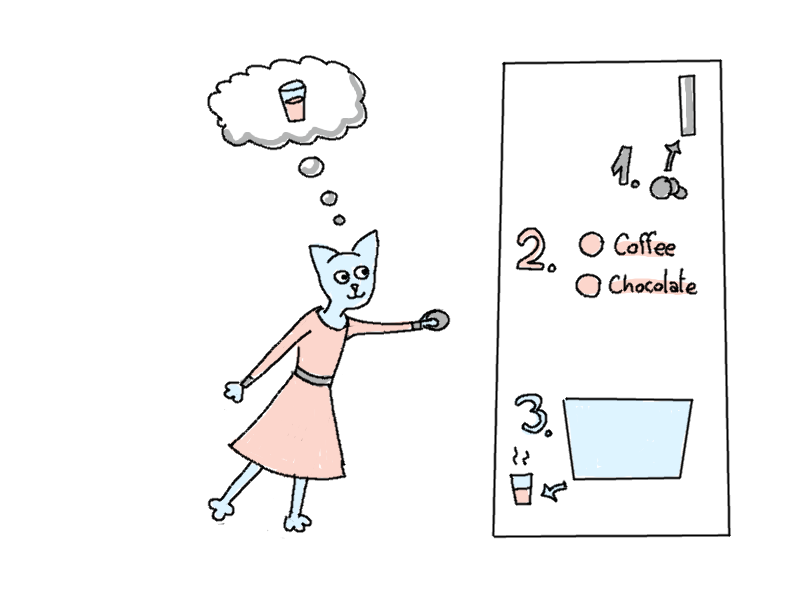
\includegraphics[width=\linewidth]{Pictures/image.png} 
\end{figure}


\section{Einführung}
Im Alltag interagieren wir mit vielen Maschinen, die sehr einfache Programme ausführen. Zum Beispiel, wie viele von euch haben heute den Lift genommen? Oder mussten an einer Ampel anstehen? Oder haben ein Getränk aus dem Automaten vor der Mensa genommen? Wie werden diese Gegenstände gesteuert?

Diese einfache Programme, die keine Variablen und keine Datenablage benötigen, nennt man \emph{endliche Automaten}. Heute werden wir Beispiele von endlichen Automaten kennenlernen und diesen Begriff genau mathematisch definieren. Auf dieser Basis werden wir dann in den nächsten Wochen aufbauen und beweisen, welche Probleme lassen sich mit solchen Programmen lösen und welche nicht.
\begin{example}
Das Beispiel mit der Ampel -- ausschreiben und zeichnen
\begin{figure}[H]
\centering
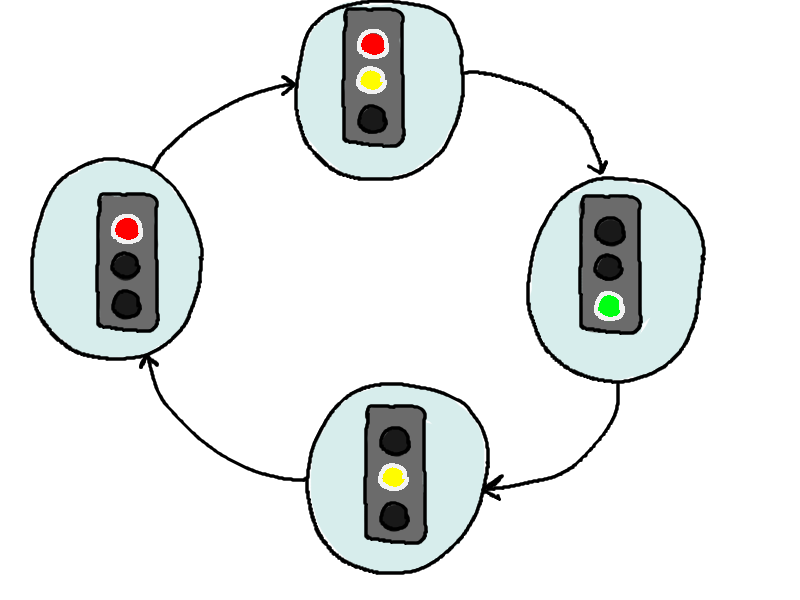
\includegraphics[width=\linewidth]{Pictures/Ampel.png} 
\end{figure}
\end{example}

\begin{example}
Das Beispiel mit dem Getränkautomat -- im Arbeitsblatt leer lassen, im Skript für Johannes und Giovanni ergänzen.
\end{example}

\begin{examplesolution}[print=true]
Das ist die Lösung. Ein schöner Automat.
\end{examplesolution}

\begin{question}
Zeichne einen Obstautomat. (Obstautomat genau beschreiben).
\end{question}

\section{Eigenschaften}
\section{Alphabeten, Wörter, Sprachen}
\begin{definition}
Eine endliche nichtleere Menge \(\sigma\) heisst \textbf{Alphabet}. Die Elemente eines Alphabets werden \textbf{Buchstaben}, \textbf{Zeichen} oder \textbf{Symbole} genannt.
\end{definition}

\begin{example}
\begin{enumerate}[(a)]
    \item \(\Sigma_{tast} = \{a, b, \dots, z, A, B, \dots, Z, 0, \dots, 9, ., ,, !, ?, -, :, \dots, @\}\) ist das Alphabet aller Zeichen, die sich mit einer Tastatur eintippen lassen. Wir benutzen dieses Alphabet, um Texte oder Programme zu schreiben.
    \item \(\Sigma_{bin} = \{0, 1\}\) ist das Alphabet, in welchem binäre Zahlen dargestellt werden.
    \item \(\Sigma_{Morse} = \{.,-\}\) ist das Alphabet der Morsezeichen.
\end{enumerate}
\end{example}

\begin{exercise}
Welche der folgenden Mengen sind Alphabete? Begründe deine Antwort.
\begin{itemize}[label=$\square$]
    \item \(\Sigma = \{a, b, C, D, e, f\}\)
    \item \(\Sigma = \{\}\)
    \item \(\Sigma = \{+, -, \times, \div\}\)
    \item \(\Sigma = \{2, 4, 6, 8, 10, 12, 14, \dots\}\), die Menge aller geraden natürlichen Zahlen
\end{itemize}
\end{exercise}

\begin{definition}
Sei \(\Sigma\) ein Alphabet. Ein \textbf{Wort über \(Sigma\)} ist eine endliche (eventuell leere) Folge von Buchstaben aus \(\Sigma\). Das \textbf{leere Wort \(\lambda\)} ist die leere Buchstabenfolge.
\end{definition}

\begin{example}
\begin{enumerate}[(a)]
    \item Sei \(\Sigma = \{a, b, c\}\). Mögliche Wörter über diesem Alphabet sind \texttt{aaaab}, \texttt{ababc}, \(\lambda\) und \texttt{a}.
    \item Sei \(\Sigma_{Morse} = \{.,-\}\). Mögliche Wörter über diesem Alphabet sind \verb|--|, \verb|---|, \verb|.-.|, \verb|...| und \verb|.|.
\end{enumerate}
\end{example}

\begin{exercise}
Welche der folgenden Buchstabenfolgen sind Wörter über dem Alphabet \(\Sigma = \{a, b, c\}\)? Begründe deine Antwort.
\begin{itemize}[label=$\square$]
    \item \texttt{abbbbcdccca}
    \item \(\lambda\)
    \item \texttt{abab}
\end{itemize}
\end{exercise}

\begin{exercise}[solution=true]
Schreibe zu jeder Symbolfolge jeweils das kleinste Alphabet \(\Sigma\), so dass die Symbolfolge ein Wort über \(\Sigma\) ist.
\begin{enumerate}[(a)]
{\setstretch{1.5}
    \item \texttt{abbabb},\hphantom{\textttt{00001}$xg(x)$} \(\Sigma = \)\blank[width=0.5\textwidth]{\(\{a,b\}\)}
    \item \(\lambda\),\hphantom{\textttt{0000100001}$xg(x)$} \(\Sigma = \)\blank[width=0.5\textwidth]{\(\{x\}\)}
    \item \texttt{01000.(00)!},\hphantom{$xg(x)$} \(\Sigma = \)\blank[width=0.5\textwidth]{\(\{0,1,.,(,),!\}\)}
    \item \texttt{aXYabwRS},\hphantom{\textttt{000}$xg(x)$} \(\Sigma = \)\blank[width=0.5\textwidth]{\(\{a,b,w,R,S,X,Y\}\)}
    
}
\end{enumerate}
\end{exercise}

\begin{definition}
Eine (eventuell leere) Menge von Wörtern über einem Alphabet \(\Sigma\) bezeichnen wir als eine \textbf{Sprache über \(\Sigma\)}. 
\end{definition}

\begin{exercise}
Bei den folgen Beispielen von Sprachen, entscheide, ob die Sprache endlich viele oder unendlich viele Wörter enthält. Ausserdem schreibe auf jeweils ein Wort über dem angegebenen Alphabet, welches in der Sprache und eins, welches \emph{nicht} in der Sprache ist.

{\setstretch{2}
\begin{enumerate}[(a)]
    \item \(L = \{x \in \{0,1\}^* \mid \abs{x}_0 \leq 3 \text{ und } \abs{x}_1 \in \{1,2\}\}\) \\
    \blank[width=\linewidth]{}

    \item \(L = \{wabba \in \{a,b\}^* \mid w \in \{a, b\}^* \text{ und } \abs(w)_a \leq 3\}\) \\
    \blank[width=\linewidth]{}
    
    \item \(L = \{1^p \mid p \text{ ist eine Primzahl}\}\) \\
    \blank[width=\linewidth]{}
    
    \item \(L = \{0^n 1^n \in \{0, 1\}^* \mid n \in \mathcal{N}\}\) \\
    \blank[width=\linewidth]{}
\end{enumerate}
}
\end{exercise}

\begin{exercise}
Schreibe die folgenden informell beschriebenen Sprachen formal als Mengen auf.


\begin{enumerate}[(a)]
    \item Die Sprache aller Wörter über \(\Sigma_{tast}\), die mit drei Ausrufezeichen enden.\\
    {\setstretch{1.5} 
    
    \blank[width=\linewidth]{}}

    \item Die Sprache aller Wörter über \(\{A, C, G, T\}\), welche höchstens 4 \(C\)'s enthalten und in denen die Summe der Anzahlen von \(A\)'s und \(G\)'s genau \(10\) ist. \\
    {\setstretch{1.5} 
    
    \blank[width=\linewidth]{}}
    
    \item Die Sprache aller Wörter über \{., -\}, welche das Teilwort \verb|...---...| enthalten. \\
    {\setstretch{1.5} 
    
    \blank[width=\linewidth]{}}
    
    \item Die Sprache aller Wörter über \{a, b, c\}, welche mit dem Präfix \(a^3 b^2 c\) anfangen. \\
    {\setstretch{1.5} 
    
    \blank[width=\linewidth]{}}
\end{enumerate}
\end{exercise}

\section{Matematische Formulierung eines endlichen Automates}
\begin{definition}[solution=true]
Ein \textbf{endlicher Automat} ist ein Quintupel \(M = (Q, \Sigma, \delta, q_0, F)\), wobei:
{\setstretch{1.5} 
\begin{enumerate}[(i)]
    \item \(Q\) \blank[width=0.5\linewidth]{eine endliche Menge von \textbf{Zuständen} ist,}
    \item \(\Sigma\) \blank[width=0.5\linewidth]{das \textbf{Eingabealphabet} ist,}
    \item \(q_0 \in Q\) \blank[width=0.5\linewidth]{der \textbf{Anfangszustand} ist,}
    \item \(F \subseteq Q\) \blank[width=0.5\linewidth]{die \textbf{Menge der akzeptierenden Zustände} ist,}
    \item \(\delta:\) \blank{\(Q\times \Sigma \rightarrow Q\)} \blank[width=0.5\linewidth]{die \textbf{Übergangsfunktion} ist.}
\end{enumerate}
}
\end{definition}


\section{Zusammenfassung}


\end{document}